\chapter{Results}
\thispagestyle{fancy}
\section{neutron-neutron Opening Angle Correlations}
The n-n opening angle correlation is calculated using the methods outlined in sec~\ref{Analysis}, in which a correlated neutron yield is divided by an uncorrelated yield.
The results are compared with output from FREYA~\cite{FREYA} (Fission Reaction Event Yield Algorithm), which was developed by the collaborative efforts of researchers from Lawrence Berkeley National Laboratory,  Lawrence Livermore National Laboratory, Los Almos National Laboratory, and University of Michigan Nuclear Engineering, and has been included in MCNP beginning with version 6.2 .
 
The most recent release of FREYA (version 2.0.3) does not model photofission directly, but instead uses a neutron-induced fission model to approximate photofission~\cite{FREYA_photofission}.
For a given nucleus with Z protons and A total nucleons, the code selects the neutron-induced fission model for a Z(A-1) nucleus, and chooses an incident neutron energy such that the compound ZA nucleus will have an excitation energy relative to the ground state of ZA that is equal to the energy of the incident photon.

When using FREYA to model photofission in this work, all model parameters, such as level density and partition parameters, were set to their default values for neutron-induced fission.
FREYA was told to use the fission fragment mass distribution, $Y(A)$, and the average total kinetic energy, $\langle$TKE$\rangle(A)$, from the $^{238}$U photofission measurements described in ref~\cite{2017Krishichayan}.
In ref~\cite{Talou2018}, the authors warn that using FREYA in this way to model photofission is only an approximation and could lead to incorrect results.
Nonetheless, FREYA is used here as such because it is the only photofission model available to the authors of the present work.

\subsection{$\theta_{\text{nn}}$ correlation \emph{versus} neutron energy}
The measured $\theta_{nn}$ distribution from the photofission of $^{238}$U and the SF of $^{252}$Cf are presented with the following three different types of cuts applied to the energies of neutrons in coincidence:
\begin{enumerate}[label=(\roman*), itemjoin={{, }}, itemjoin*={{, or }}]
    \item In Figs.~\ref{fig:DU(0)} ($^{238}$U) and~\ref{fig:Cf(0)} ($^{252}$Cf), a minimum energy threshold is applied to both neutrons
    \item In Figs.~\ref{fig:DU(2)} ($^{238}$U) and~\ref{fig:Cf(2)} ($^{252}$Cf), the energy of both neutrons are required to fall within a specified range
  \item In Figs.~\ref{fig:DU(1)} ($^{238}$U) and~\ref{fig:Cf(1)} ($^{252}$Cf), the mean energy of the two neutrons are required to fall within a specified range
 \end{enumerate}

When using a histogram to estimate a continuous distribution from the relatively small number of data points obtained in this work, one faces the following dilemma: small bins produce histograms with large uncertainties that are dependent on the chosen bin-width, while large bins obscure potentially useful information. 
For this reason, kernel density estimates (KDE) with 68\% confidence intervals are plotted alongside histograms.
A KDE is a method for estimating a continuous probability distribution from a finite set of sampled data points.
The kernel was chosen to be the measurement errors in opening angle as determined by a study using a collimated $^{60}$Co source that was placed at different points along a detector.
The measurement errors in $\theta_{nn}$ are well-described by a gaussian with a sigma of 6$^{\circ}$.
Mathematical details of the KDE method used in this work are outlined in ref~\cite{KDE}. 

Plotted alongside each measurement is the result of a FREYA simulation.
For $^{238}$U photofission, there were a total of 2,952 n-n coincident events after the subtraction of accidentals and 21,882 for $^{252}$Cf SF.

\FloatBarrier
\begin{figure}
\centering
    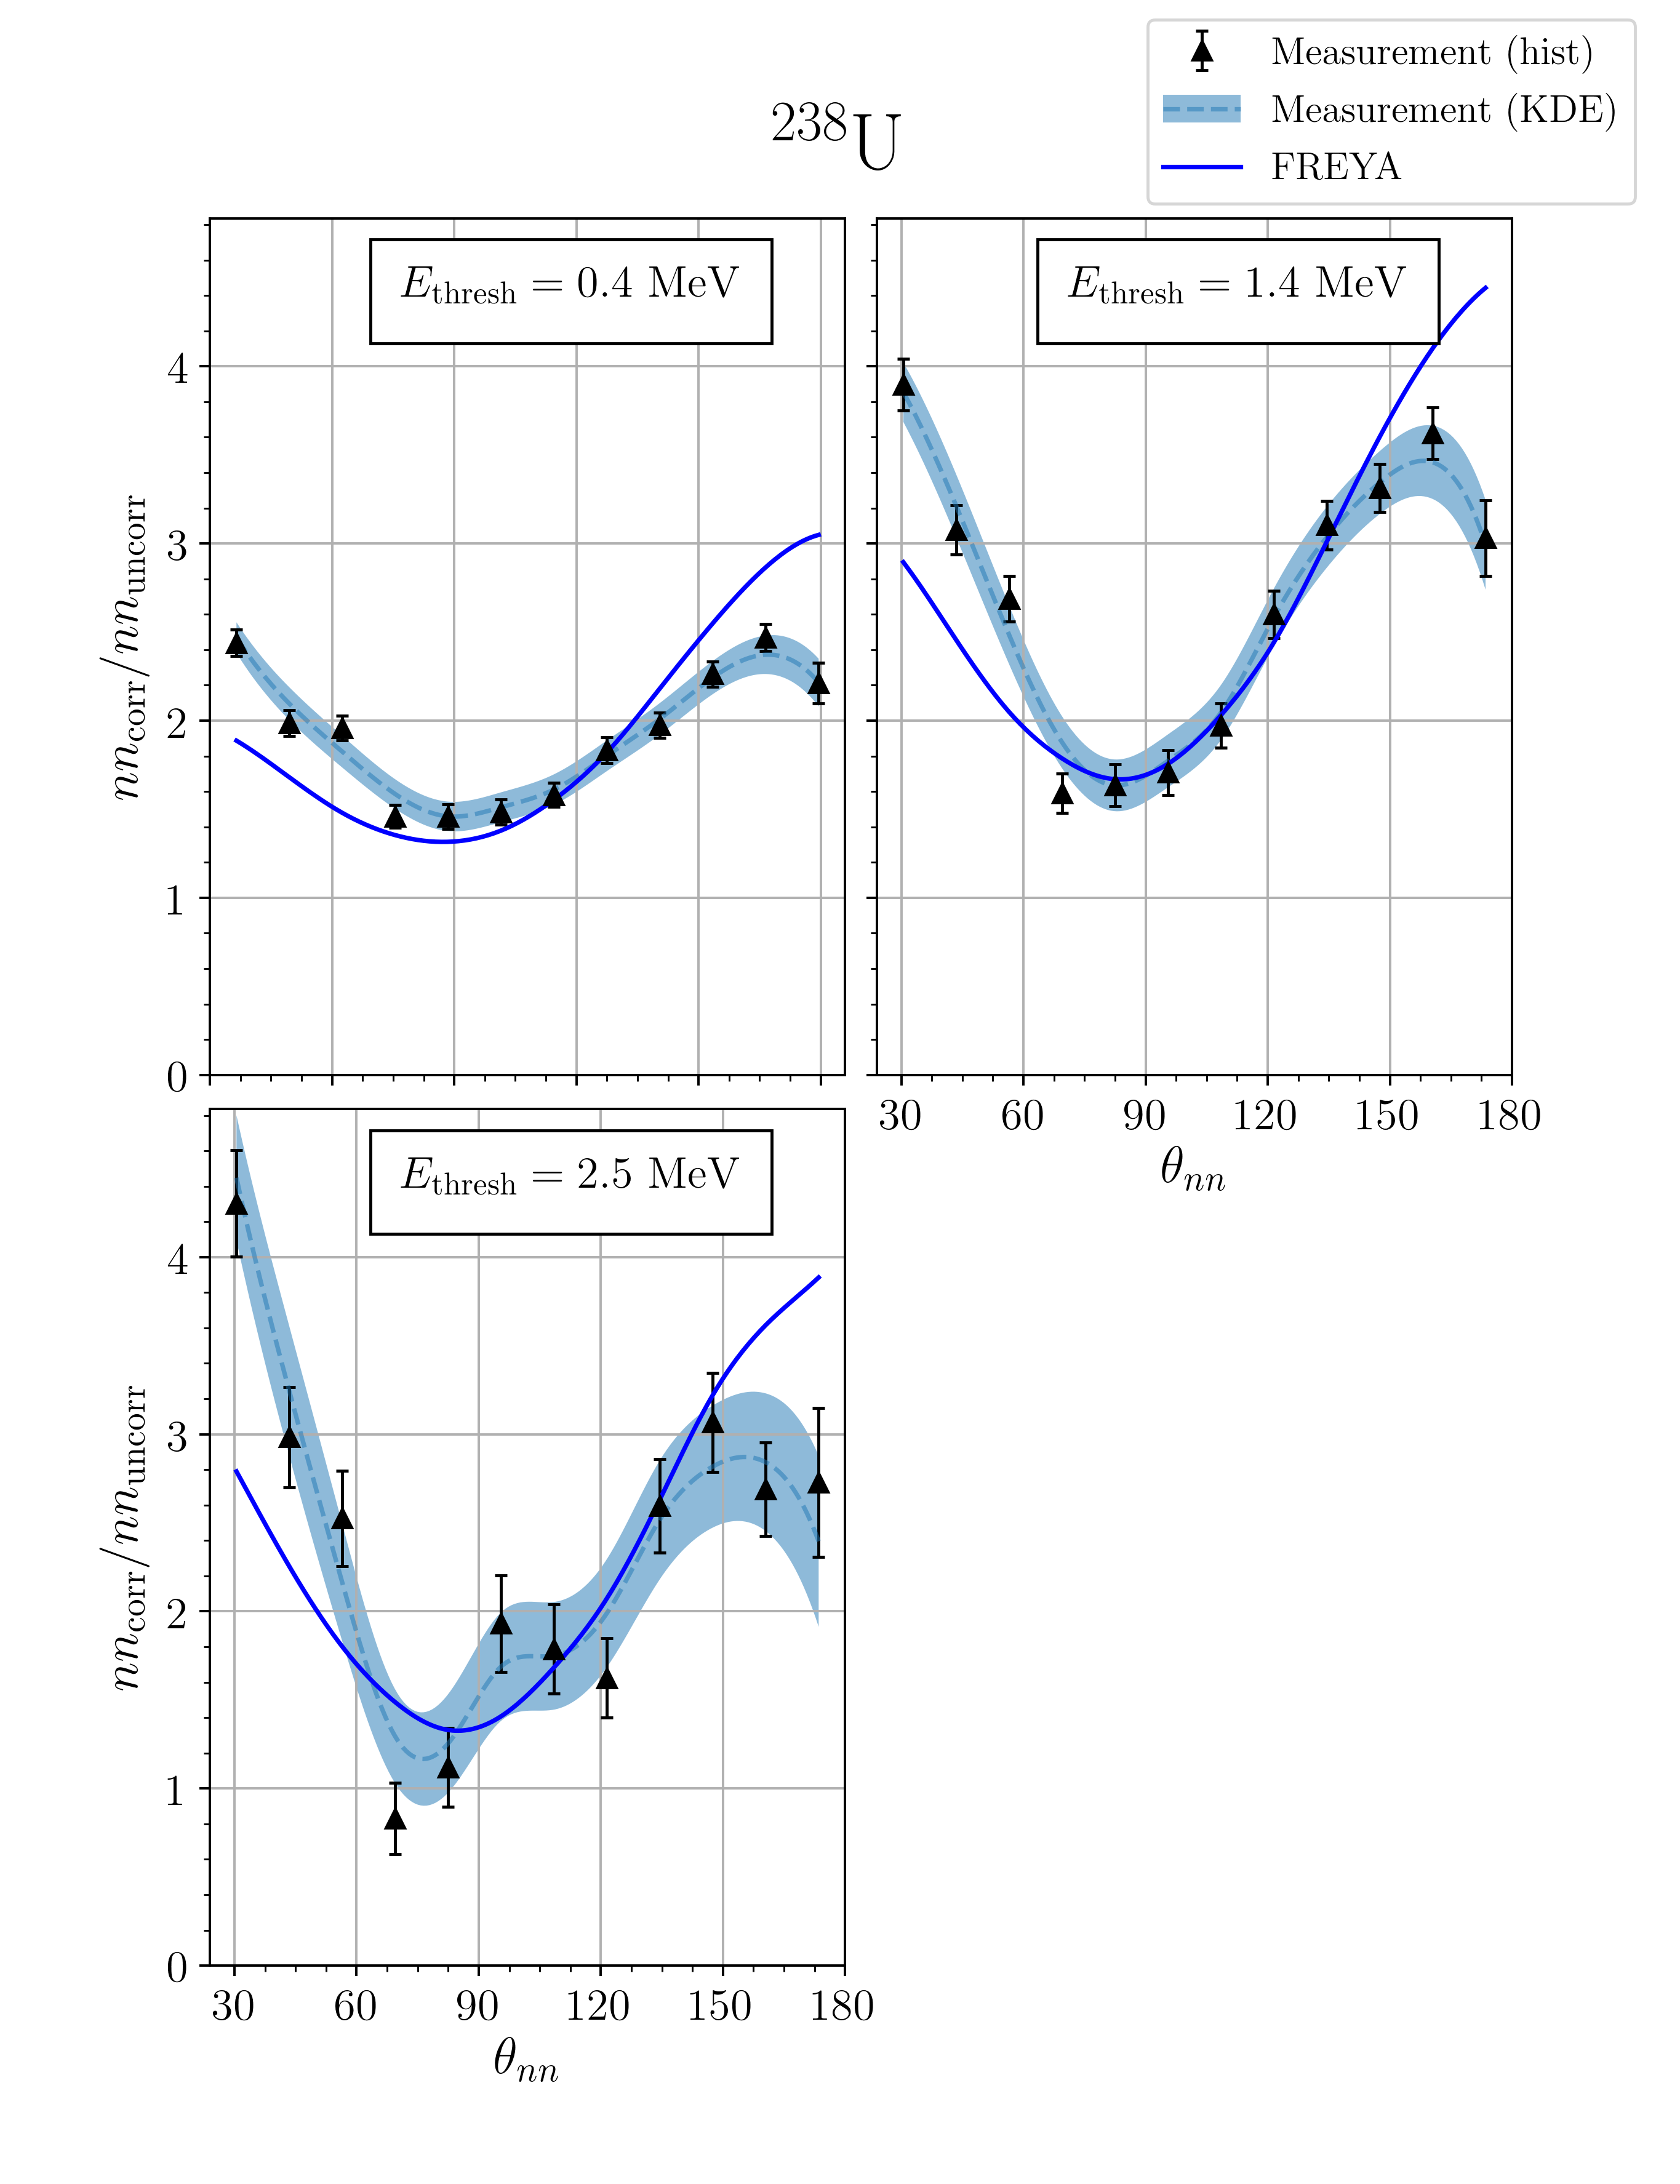
\includegraphics[width = 1.1\textwidth]{Content/Results/FinalDUResultw_freya0KDE.png}
    \caption{$\theta_{nn}$ distribution with minimum energy threshold cuts applied to all neutrons.
    The number of events contributing to each plot are, starting from the lower left and moving clockwise: 314, 2952, and 1489 .}
    \label{fig:DU(0)}
\end{figure}
\begin{figure}
\centering
    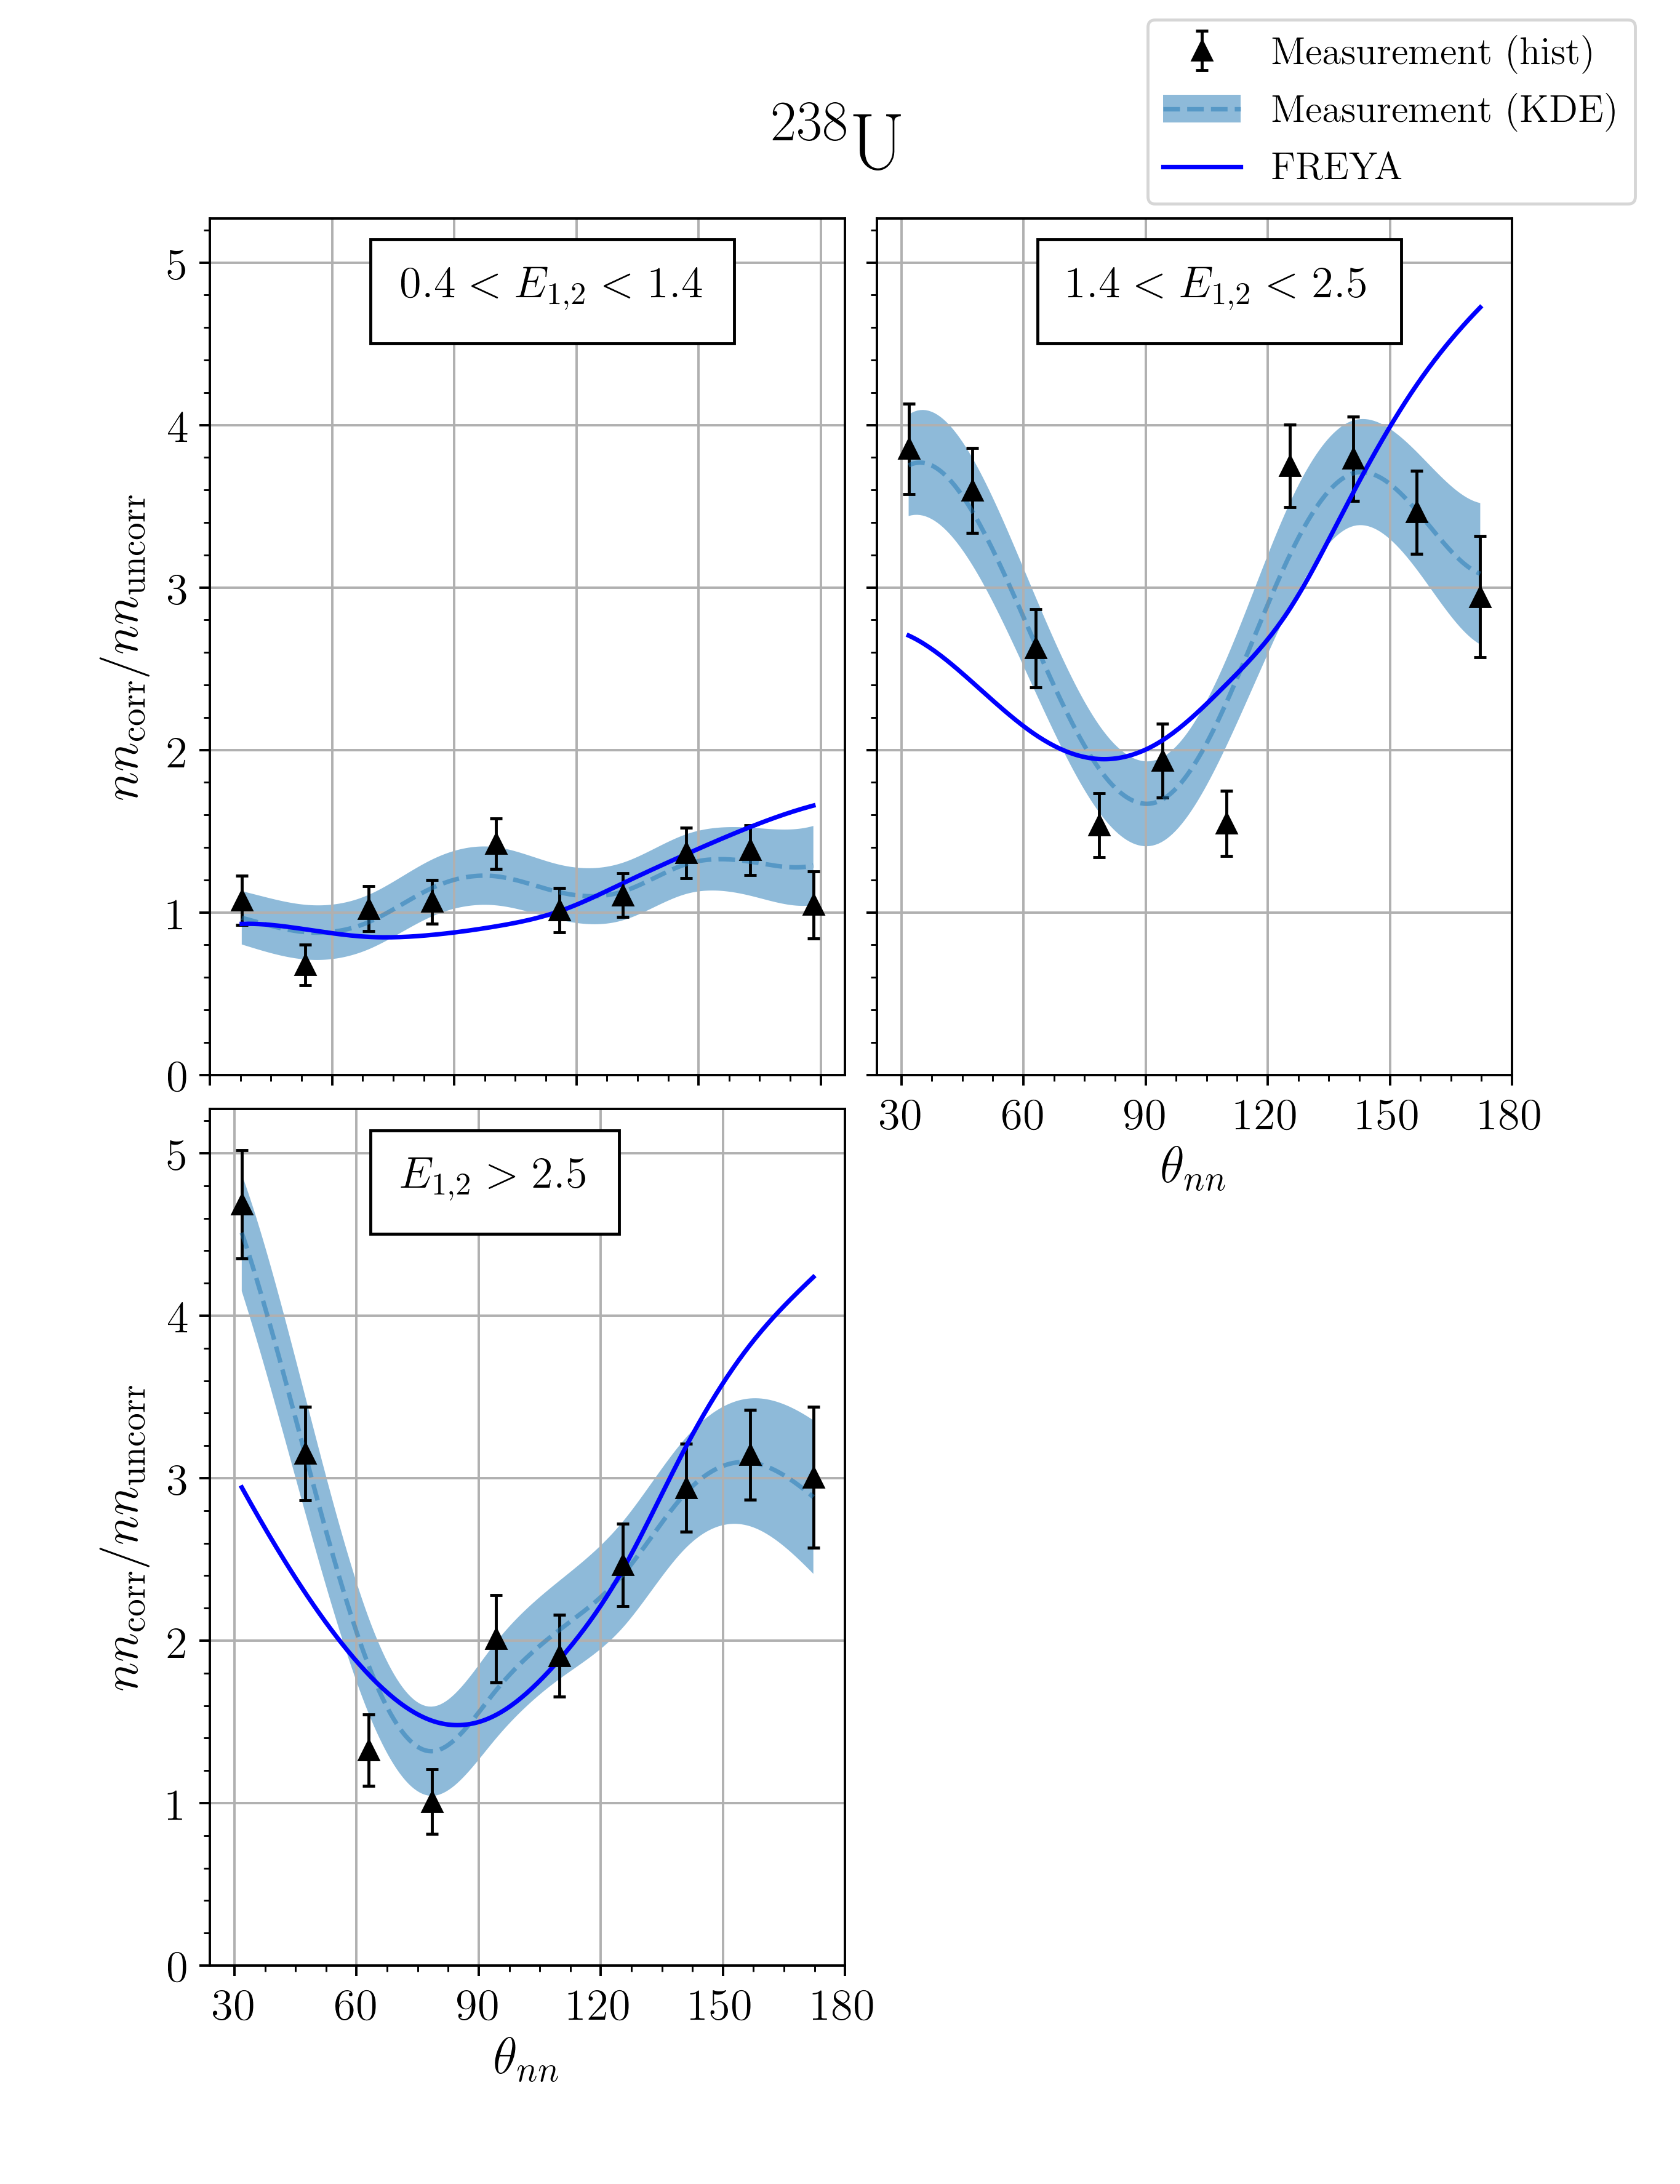
\includegraphics[width = 1.1\textwidth]{Content/Results/FinalDUResultw_freya2KDE.png}
    \caption{ $\theta_{nn}$ distribution with cuts requiring that the energy of both coincident neutrons be within the specified range.
    The number of events contributing to each plot are, starting from the lower left and moving clockwise: 303, 266, and 433 .}
    \label{fig:DU(2)}
\end{figure}
\begin{figure}
\centering
    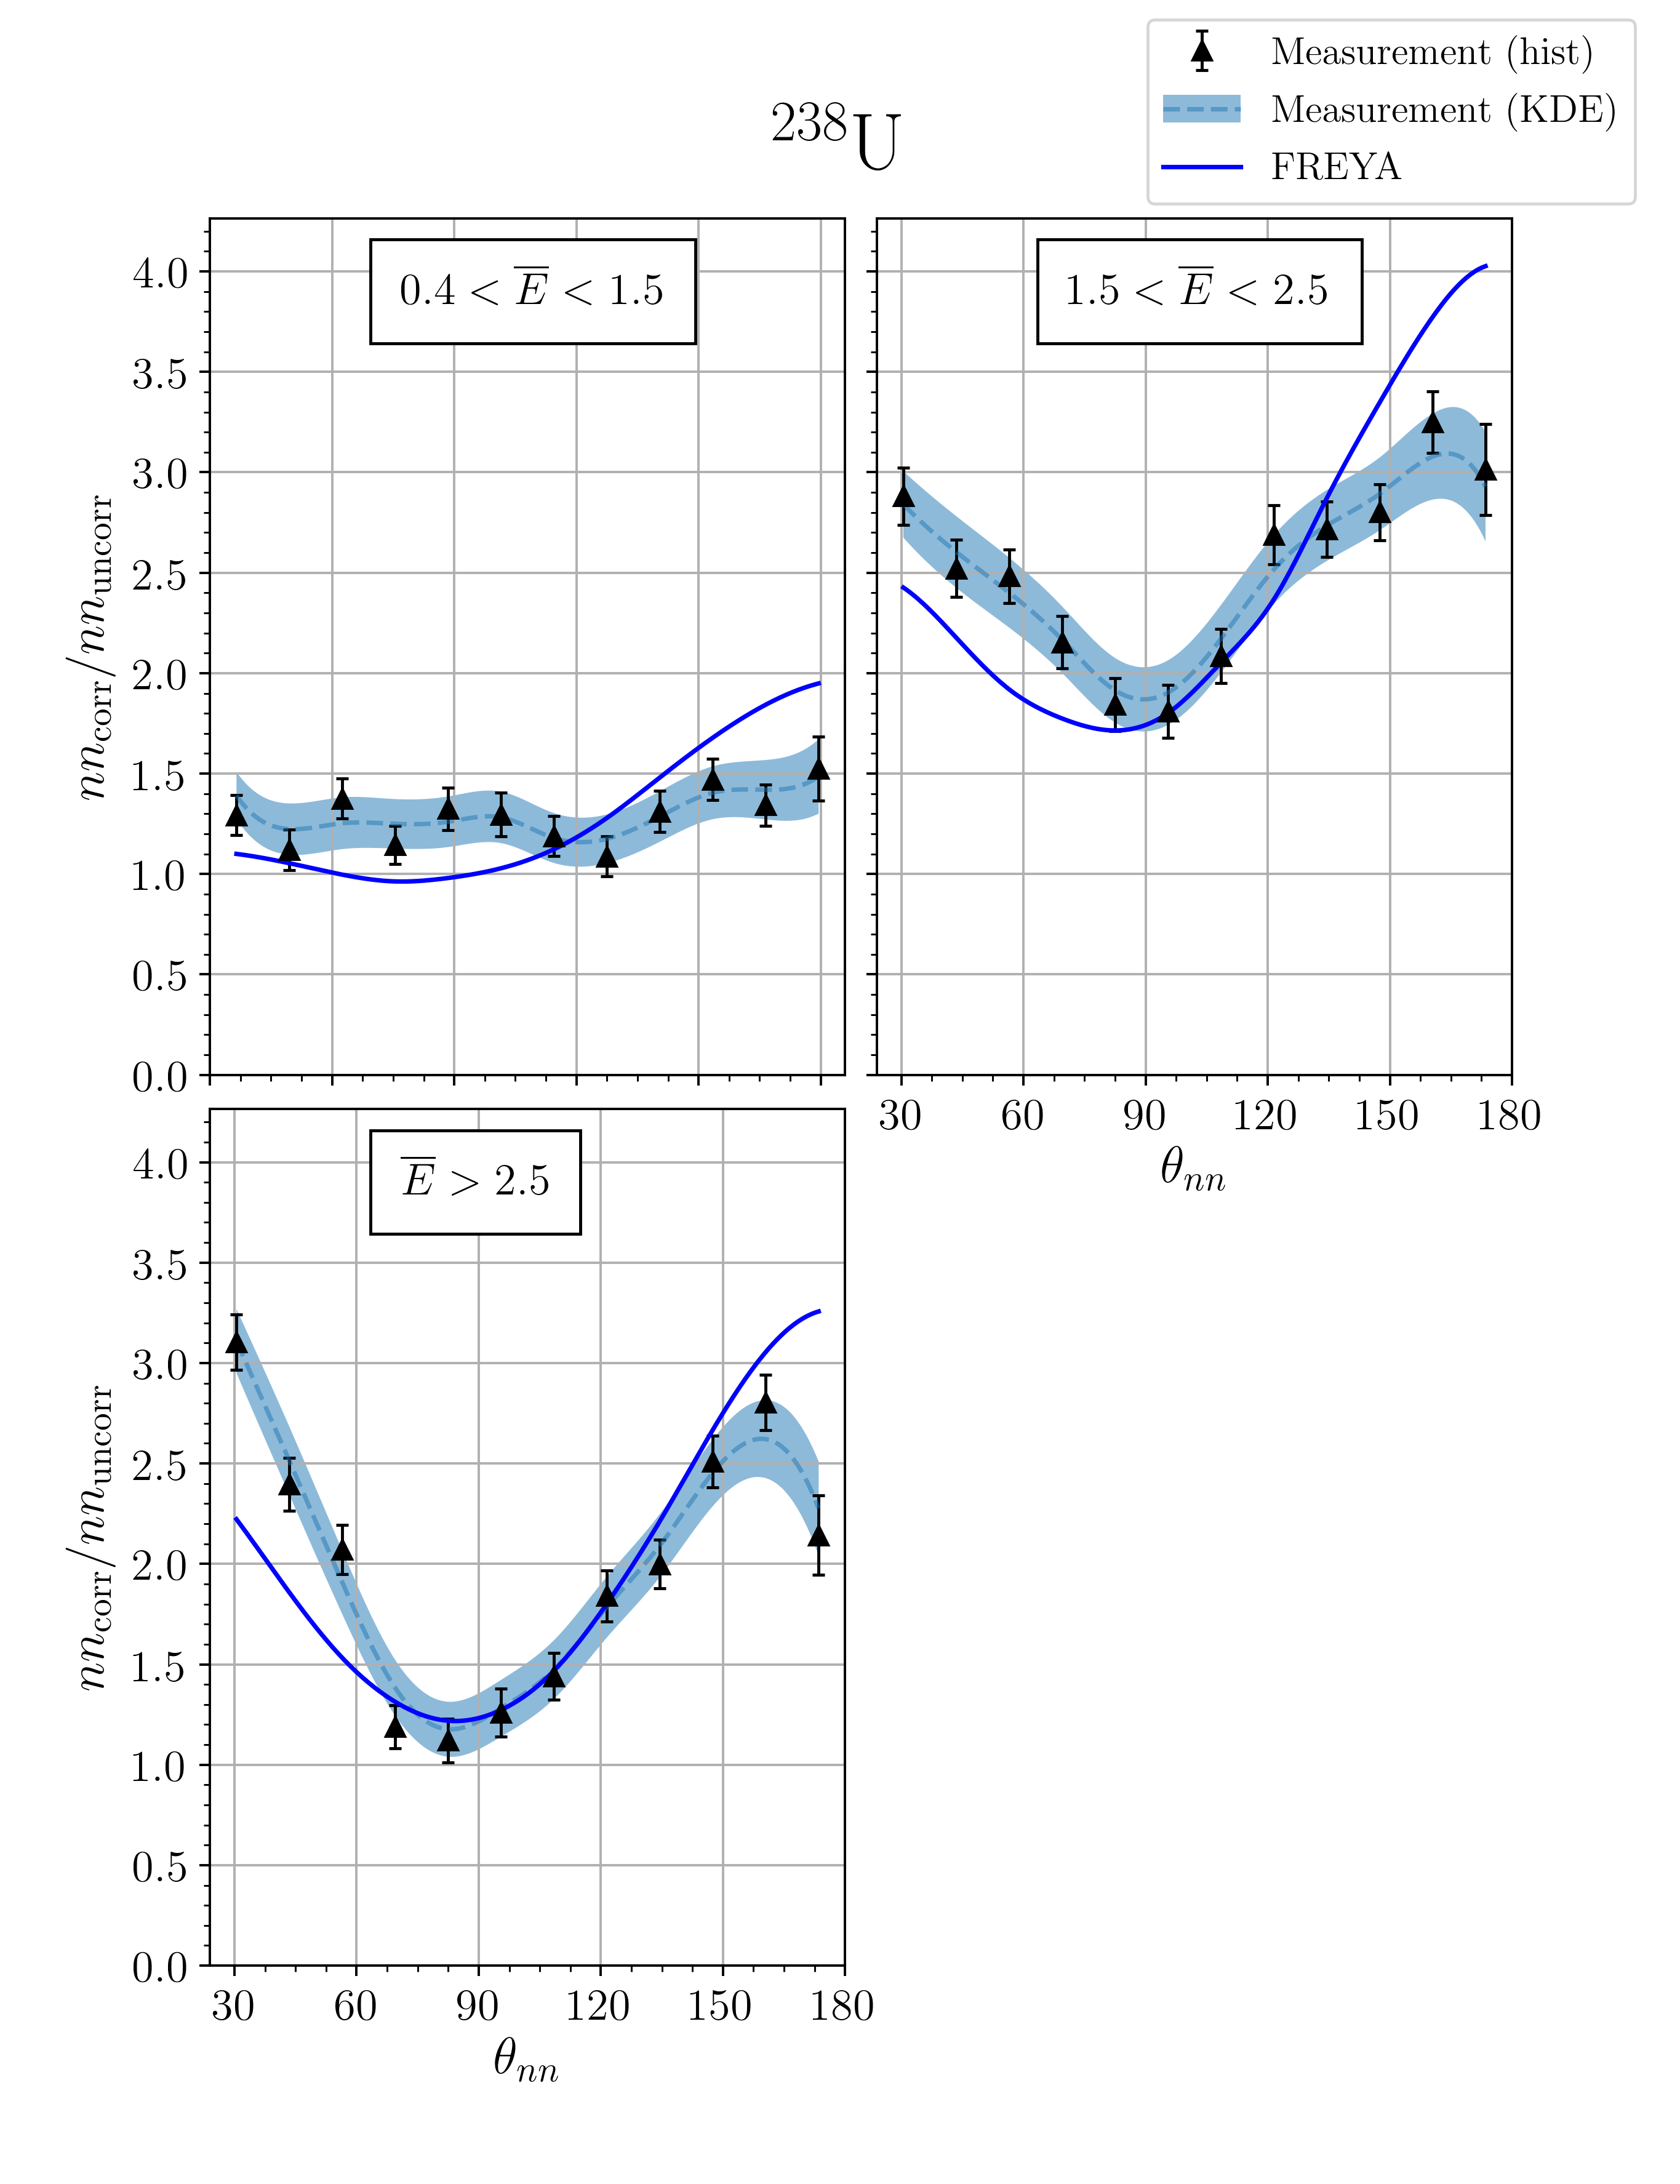
\includegraphics[width = 1.1\textwidth]{Content/Results/FinalDUResultw_freya1KDE.png}
    \caption{$\theta_{nn}$ distribution with cuts on the mean energy ($\overline{E}$) of the two coincident neutrons.
    The number of events contributing to each plot are, starting from the lower left and moving clockwise: 1009, 756, 1187 .}
    \label{fig:DU(1)}
\end{figure}
\begin{figure}
\centering
    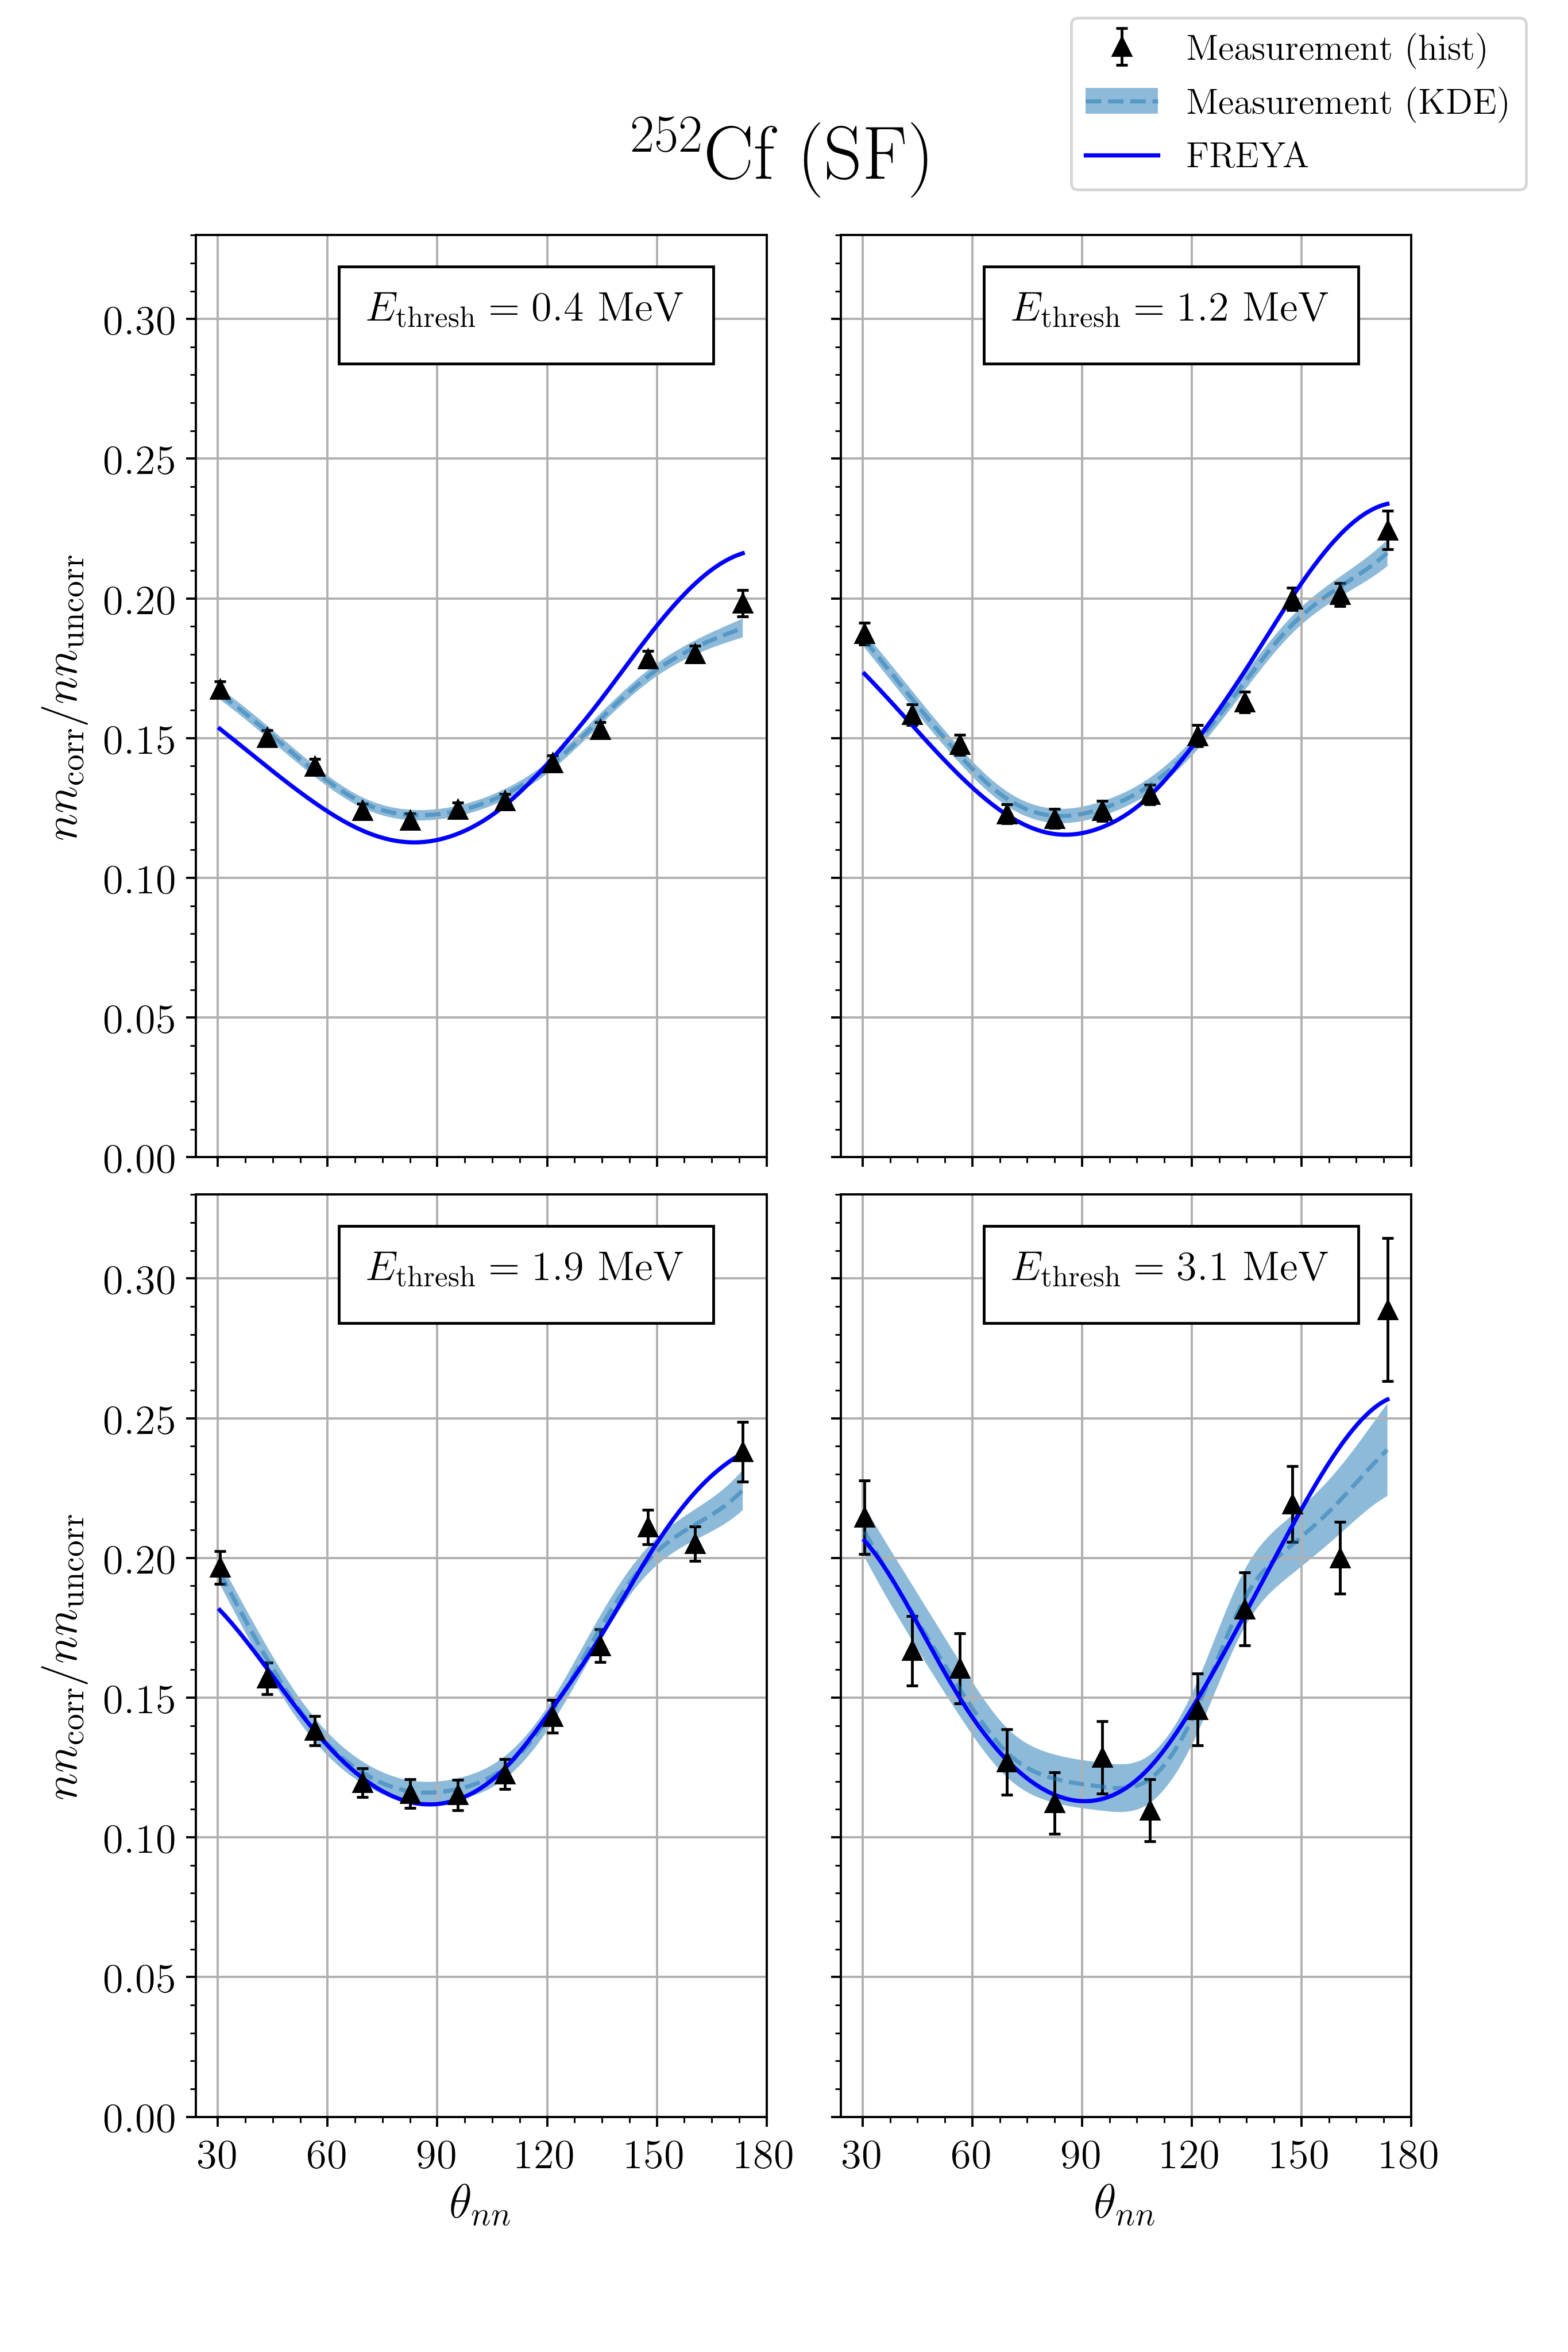
\includegraphics[width = \textwidth]{Content/Results/FinalCf252Resultw_freya0KDE.png}
    \caption{
    $\theta_{nn}$ distribution a minimum energy threshold cuts applied to all neutrons.
    The number of events contributing to each plot are, starting from the lower left and moving clockwise: 21882, 12519, 5451, 1262 .}
    \label{fig:Cf(0)}
\end{figure}
\begin{figure}
\centering
    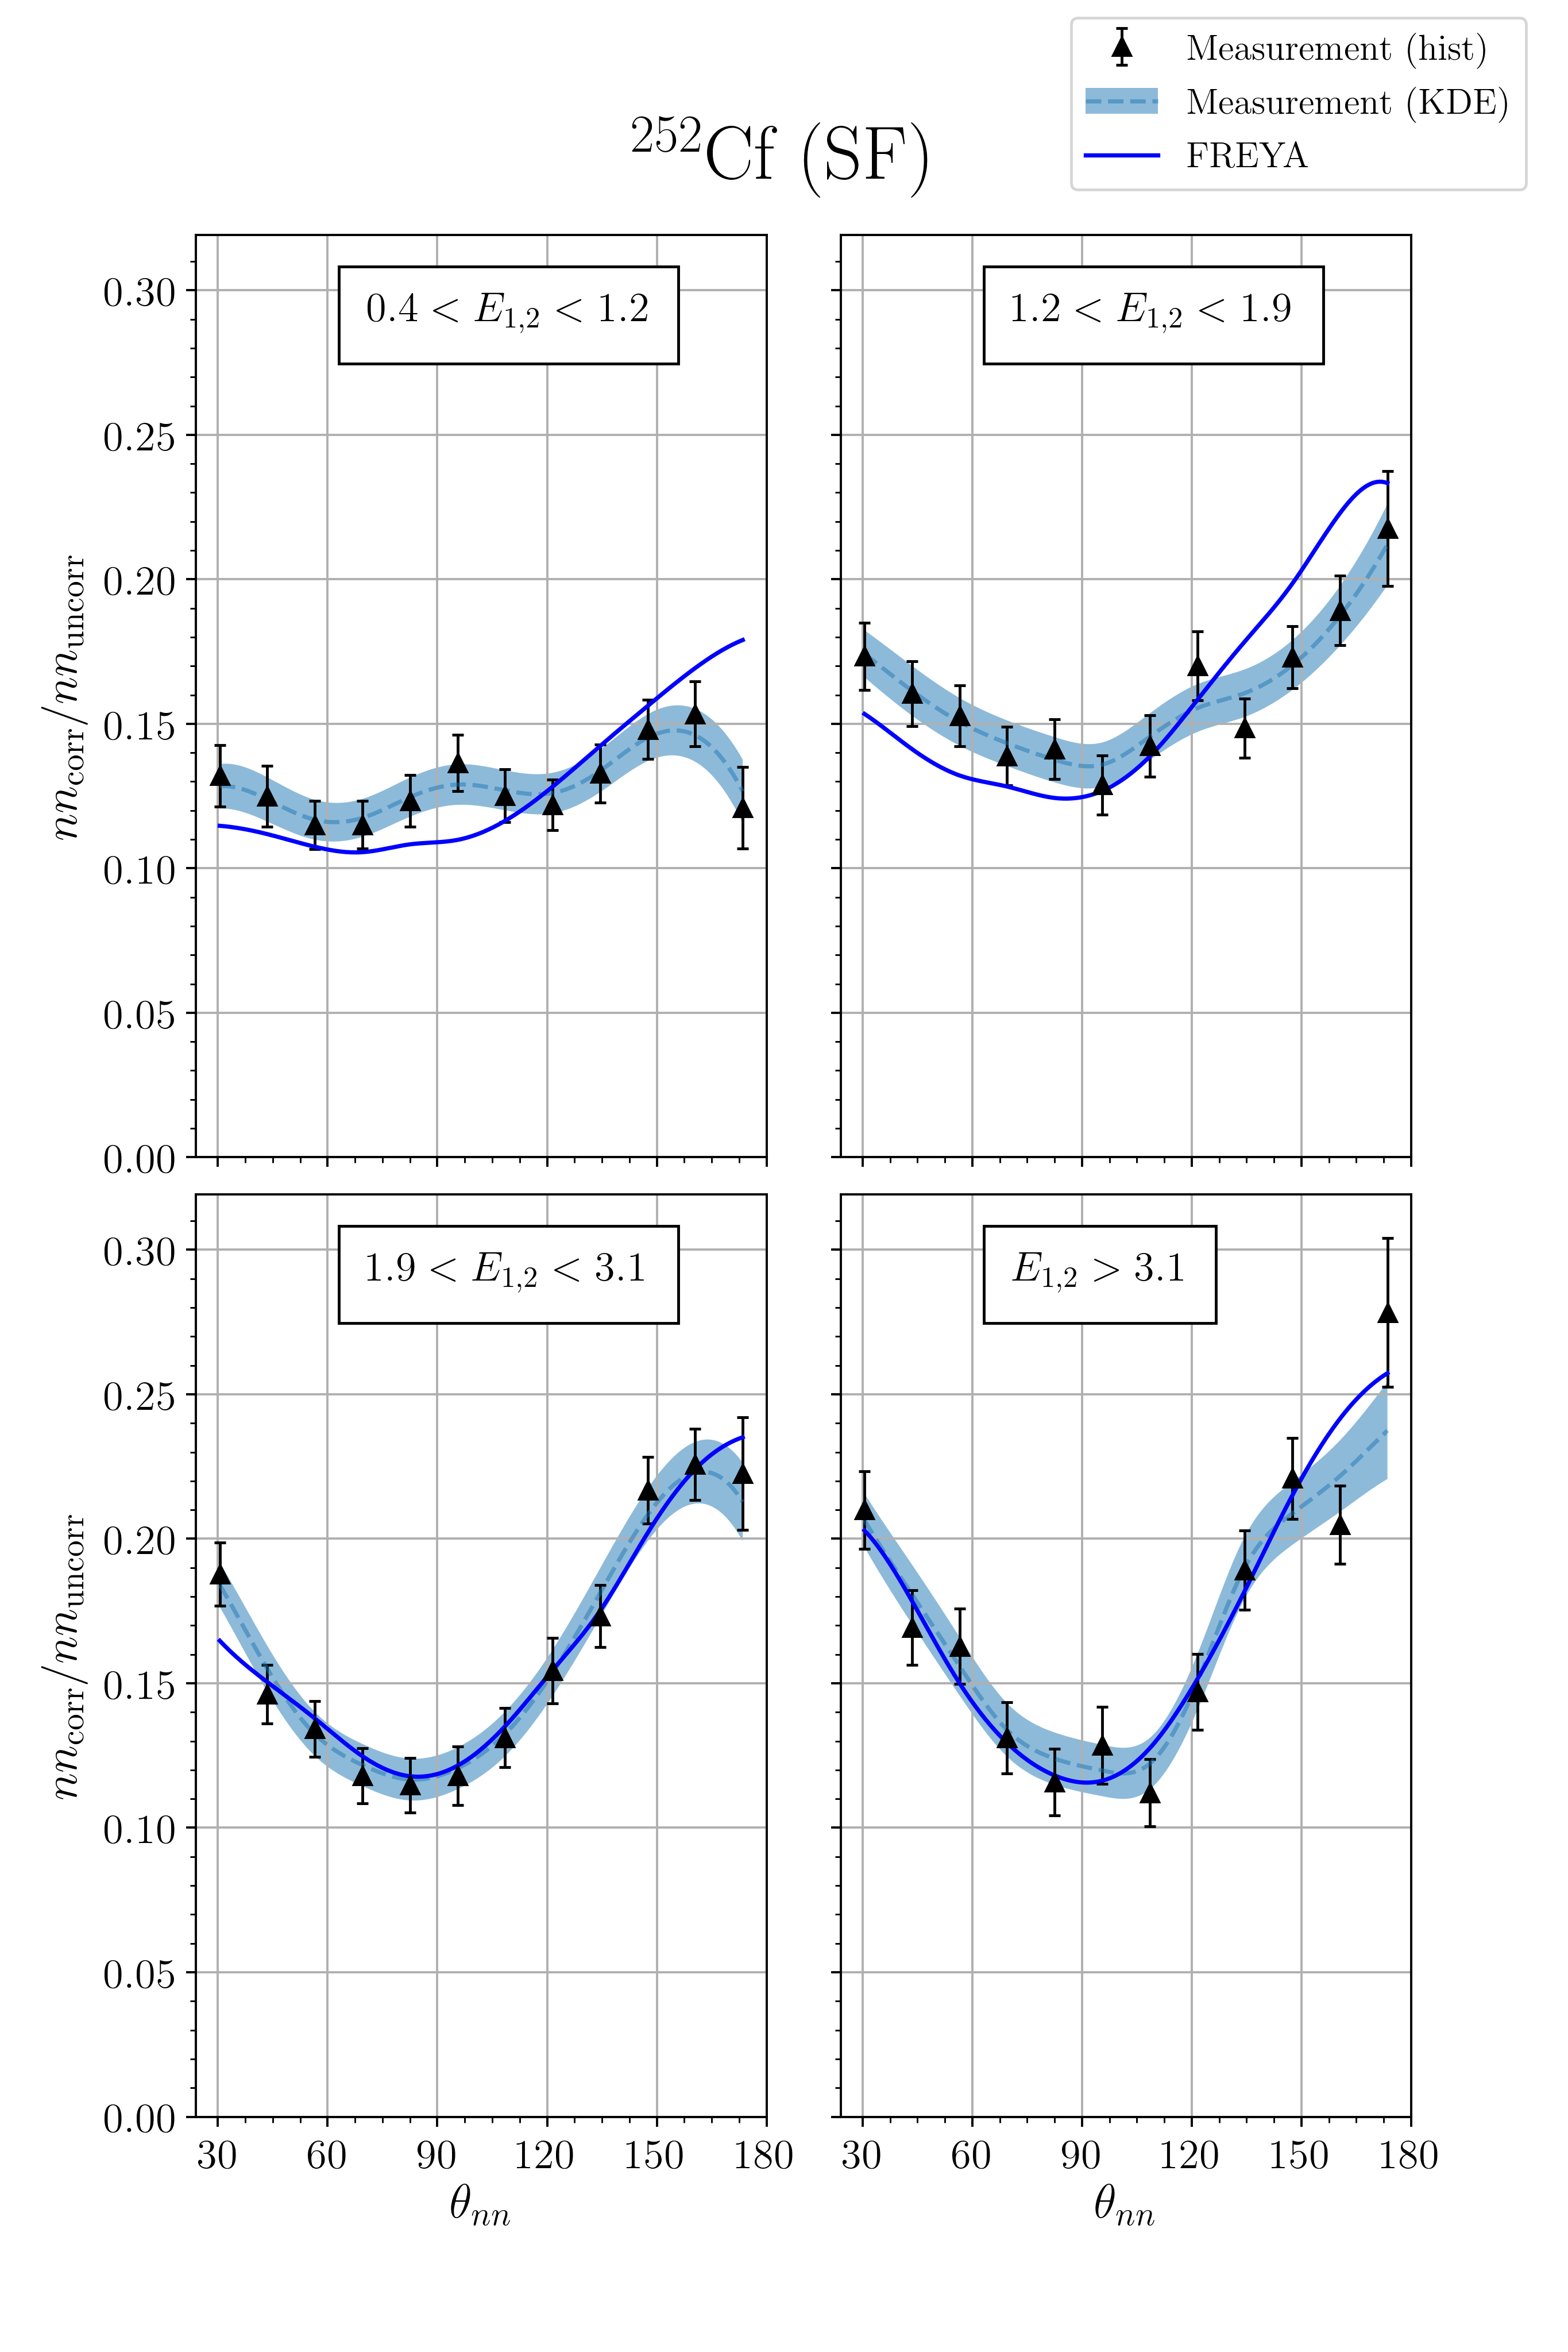
\includegraphics[width = \textwidth]{Content/Results/FinalCf252Resultw_freya2KDE.png}
    \caption{$\theta_{nn}$ distribution with cuts requiring that the energy of both coincident neutrons be within the specified range.
    The number of events contributing to each plot are, starting from the lower left and moving clockwise: 1291, 1456, 1567, 1198 .}
    \label{fig:Cf(2)}
\end{figure}
\begin{figure}
\centering
    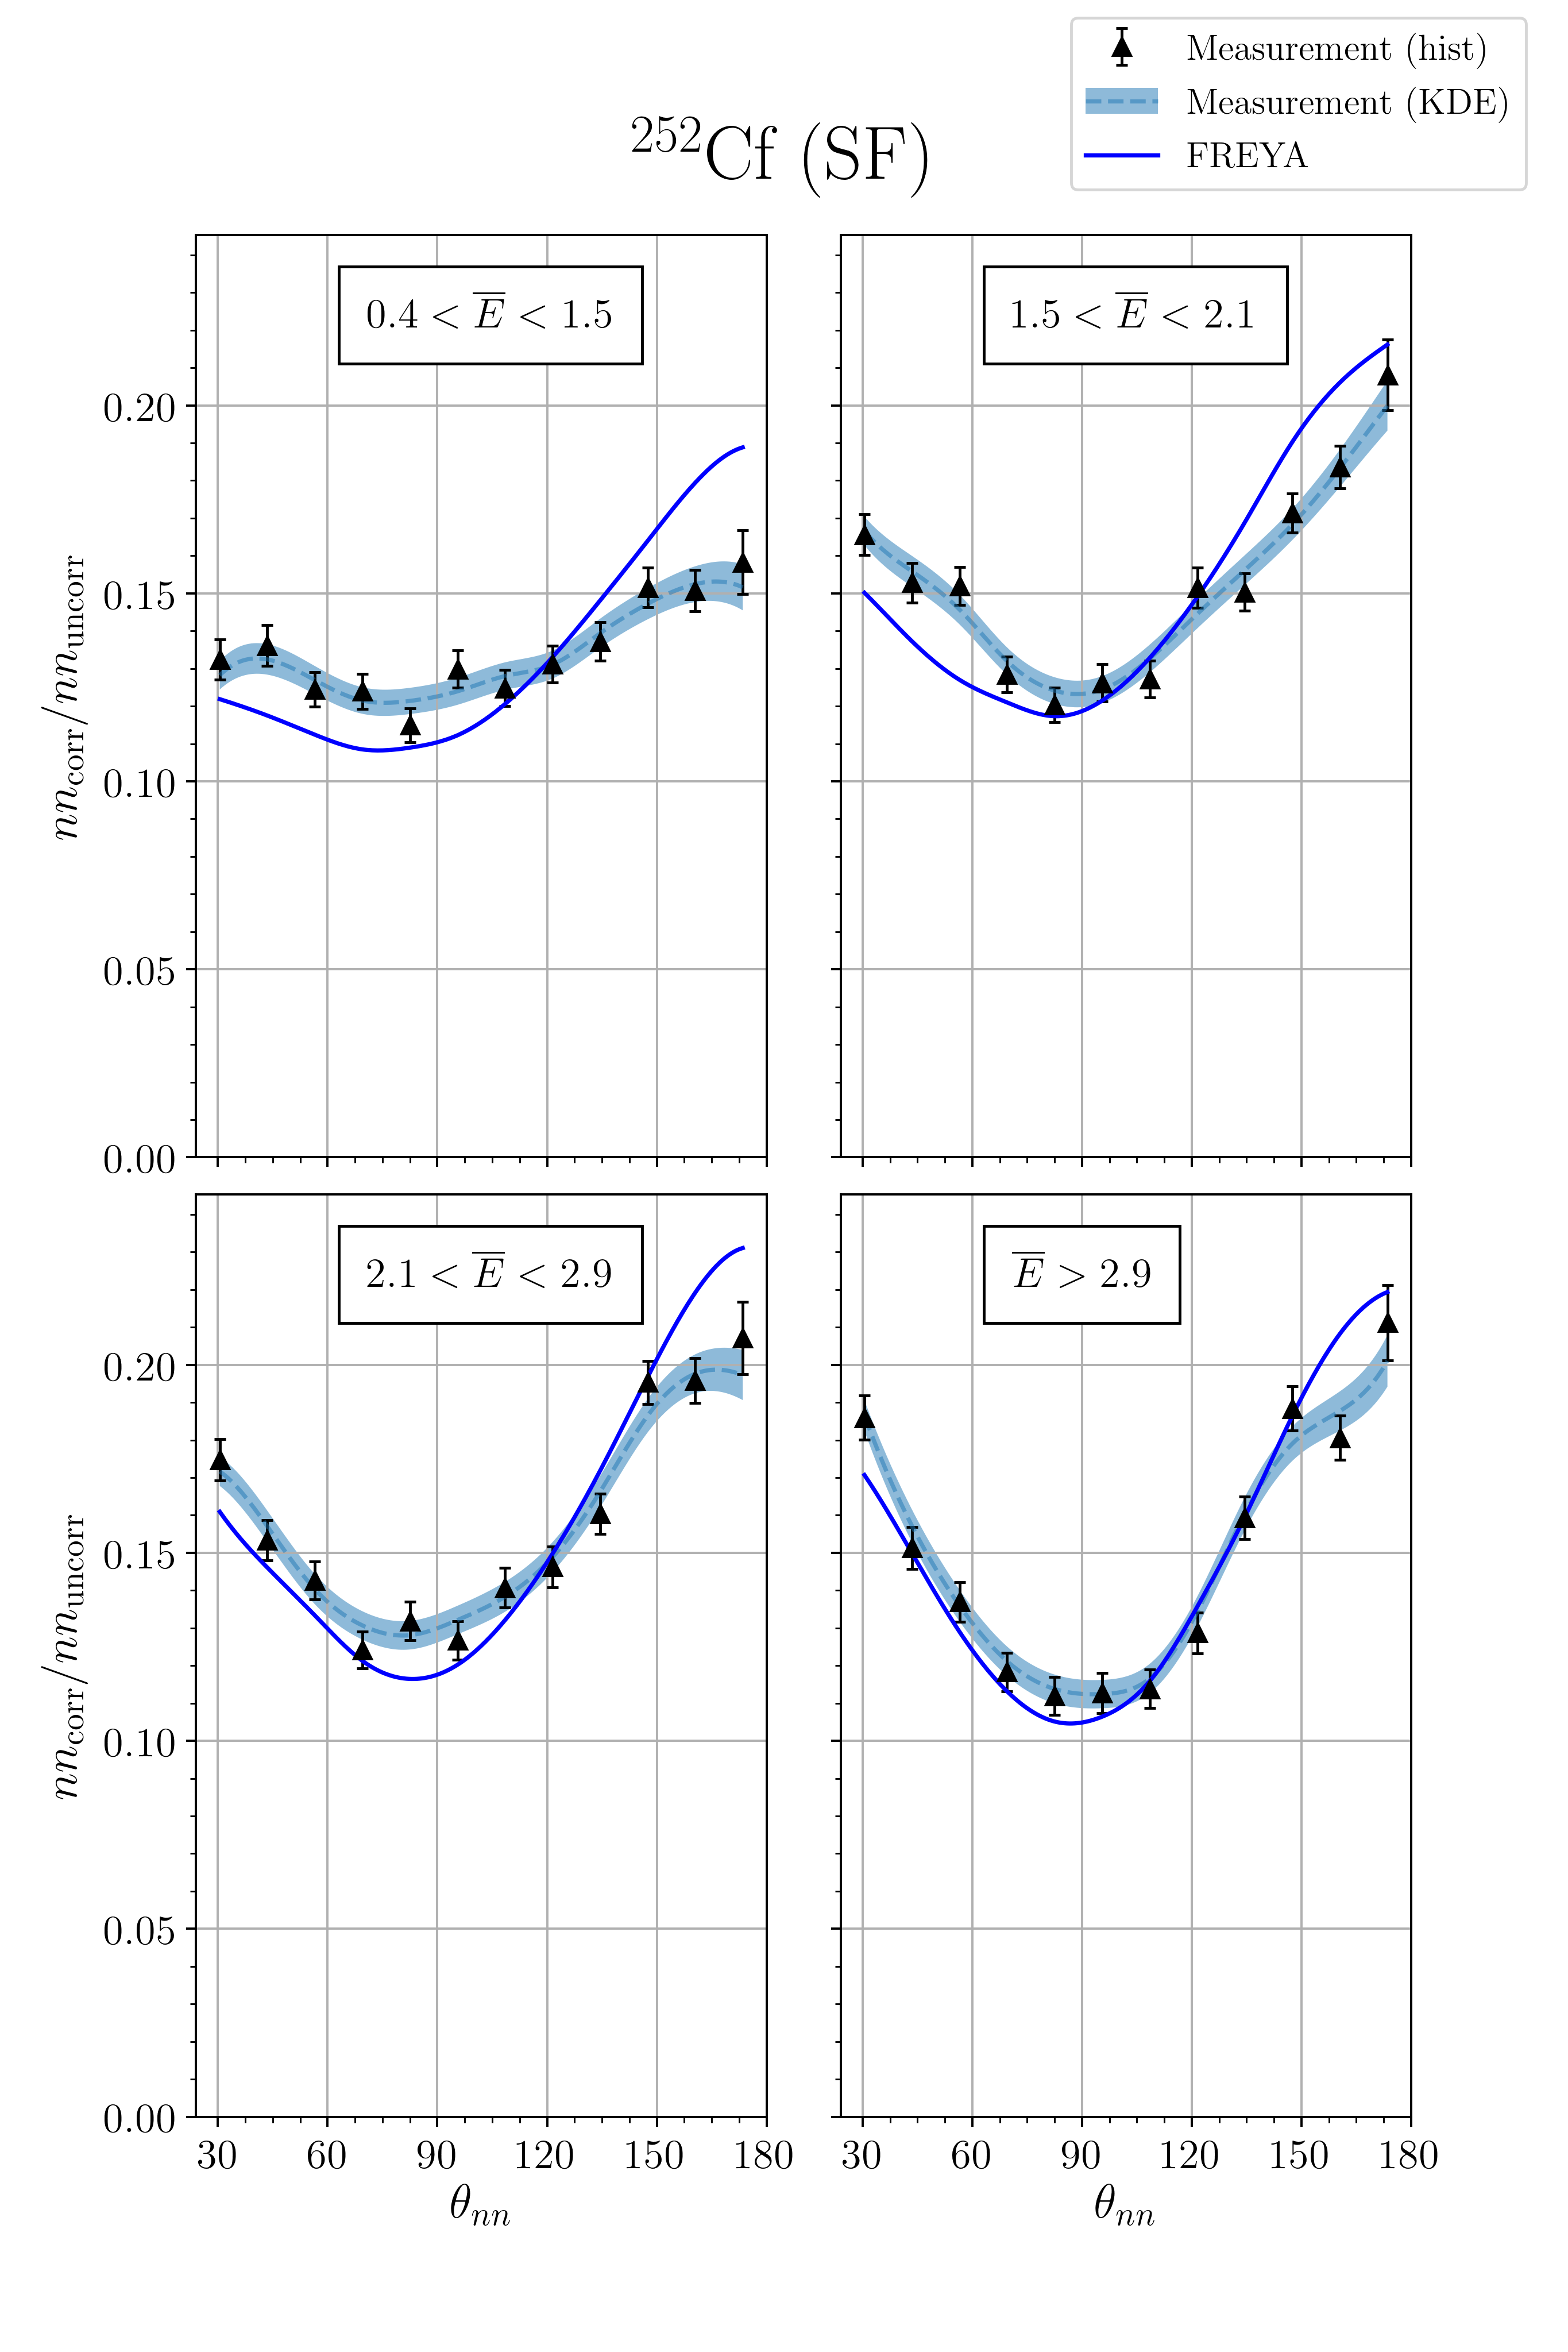
\includegraphics[width = \textwidth]{Content/Results/FinalCf252Resultw_freya1KDE.png}
    \caption{$\theta_{nn}$ distribution with cuts on the mean energy ($\overline{E}$) of the two coincident neutrons.
   The number of events contributing to each plot are, starting from the lower left and moving clockwise: 4974, 5947, 5908, 5053 . }
    \label{fig:Cf(1)}
\end{figure}
\FloatBarrier

\subsection{Considering $\theta_{abs}$}
\label{sec:anomaly}
While these results are consistent with the effect of the kinematic focusing of the neutrons due to the recoil of the fission fragments, the data show a marked decrease in the n-n opening angle correlation in the region from about 165$^{\circ}$ to 180$^{\circ}$, which can be seen in Figs.~\ref{fig:SPDPNormalization} and ~\ref{fig:theta_abs_two_neutron}, as well as in Figs ~\ref{fig:DU(0)} through \ref{fig:DU(1)}.
This feature is not evident in previous work on spontaneous and neutron induced fission.
As previously discussed in section~\ref{sec:level1}, photofission differs from spontaneous and neutron induced fission in that the fission fragments for the photon-induced reaction exhibit an asymmetry in their angle of emission, with the most likely orientation of the fission axis lying perpendicular to the direction of the incident photon.
With this in mind, the following series of angular cuts were made on the data.
Fig.~\ref{fig:theta_abs_LEGO} shows the distributions of absolute opening angles of the n-n events for three different cuts on the value of the n-n opening angle.
For n-n opening angles between 120$^{\circ}$ and 160$^{\circ}$, there is an increased preponderance of both neutrons being emitted around 90$^{\circ}$, consistent with the interpretation of kinematic focusing of neutrons coming from fission fragments which are themselves being emitted preferentially at 90$^{\circ}$.
However, in the opening angle region where the n-n correlation is reduced, from about 160$^{\circ}$ to 180$^{\circ}$, this feature is less prominent.

Furthermore, if one plots the opening angle distributions for the case in which at least one neutron is emitted perpendicular to the incident photon \emph{versus} the case in which neither neutron is emitted perpendicular to the incident photon (Fig.~\ref{fig:theta_abs_two_neutron}), one sees distinct differences.
The fact that there are overall differences is not surprising, because in one case (Fig.~\ref{fig:theta_abs_two_neutron} left) at least one neutron preferentially receives a kinematic boost from a fission fragment and in the other case (Fig.~\ref{fig:theta_abs_two_neutron} right) neither neutron does.
However, the fact that the n-n correlation is reduced at 180$^{\circ}$ in opening angle when at least one of the neutrons is emitted along the preferred fission axis is unexpected.
This is a feature which does not seem to appear in either neutron-induced fission, previous measurements on spontaneous fission, or our present measurement on spontaneous fission.
The photofission of the even-even $^{238}$U nucleus seems to be unique in this regard. 
The attribution of this effect to the geometric coverage of the neutron detection system or to neutron elastic scattering within the target was ruled out using simulations, as discussed in section~\ref{subsection:Elastic_scattering}.

These data are consistent with two possible explanations relating to the unique feature of the asymmetric angular emission of fission fragments in photofission.
First, it is possible that there is a decrease in neutron emission along the fission axis.
Second, the neutrons may indeed be emitted isotropically in the rest frame of the fission fragment, but one fragment essentially shadows the neutrons emitted from the other fragment, either through absorption or scattering.
If it is the later case, then this effect has the potential to shed light on the time dependence of neutron emission, since shadowing would likely depend on the fission fragment separation.
A definitive interpretation of this decreased n-n correlation for large opening angles in photo-fission requires further study.

\begin{figure}
\centering
    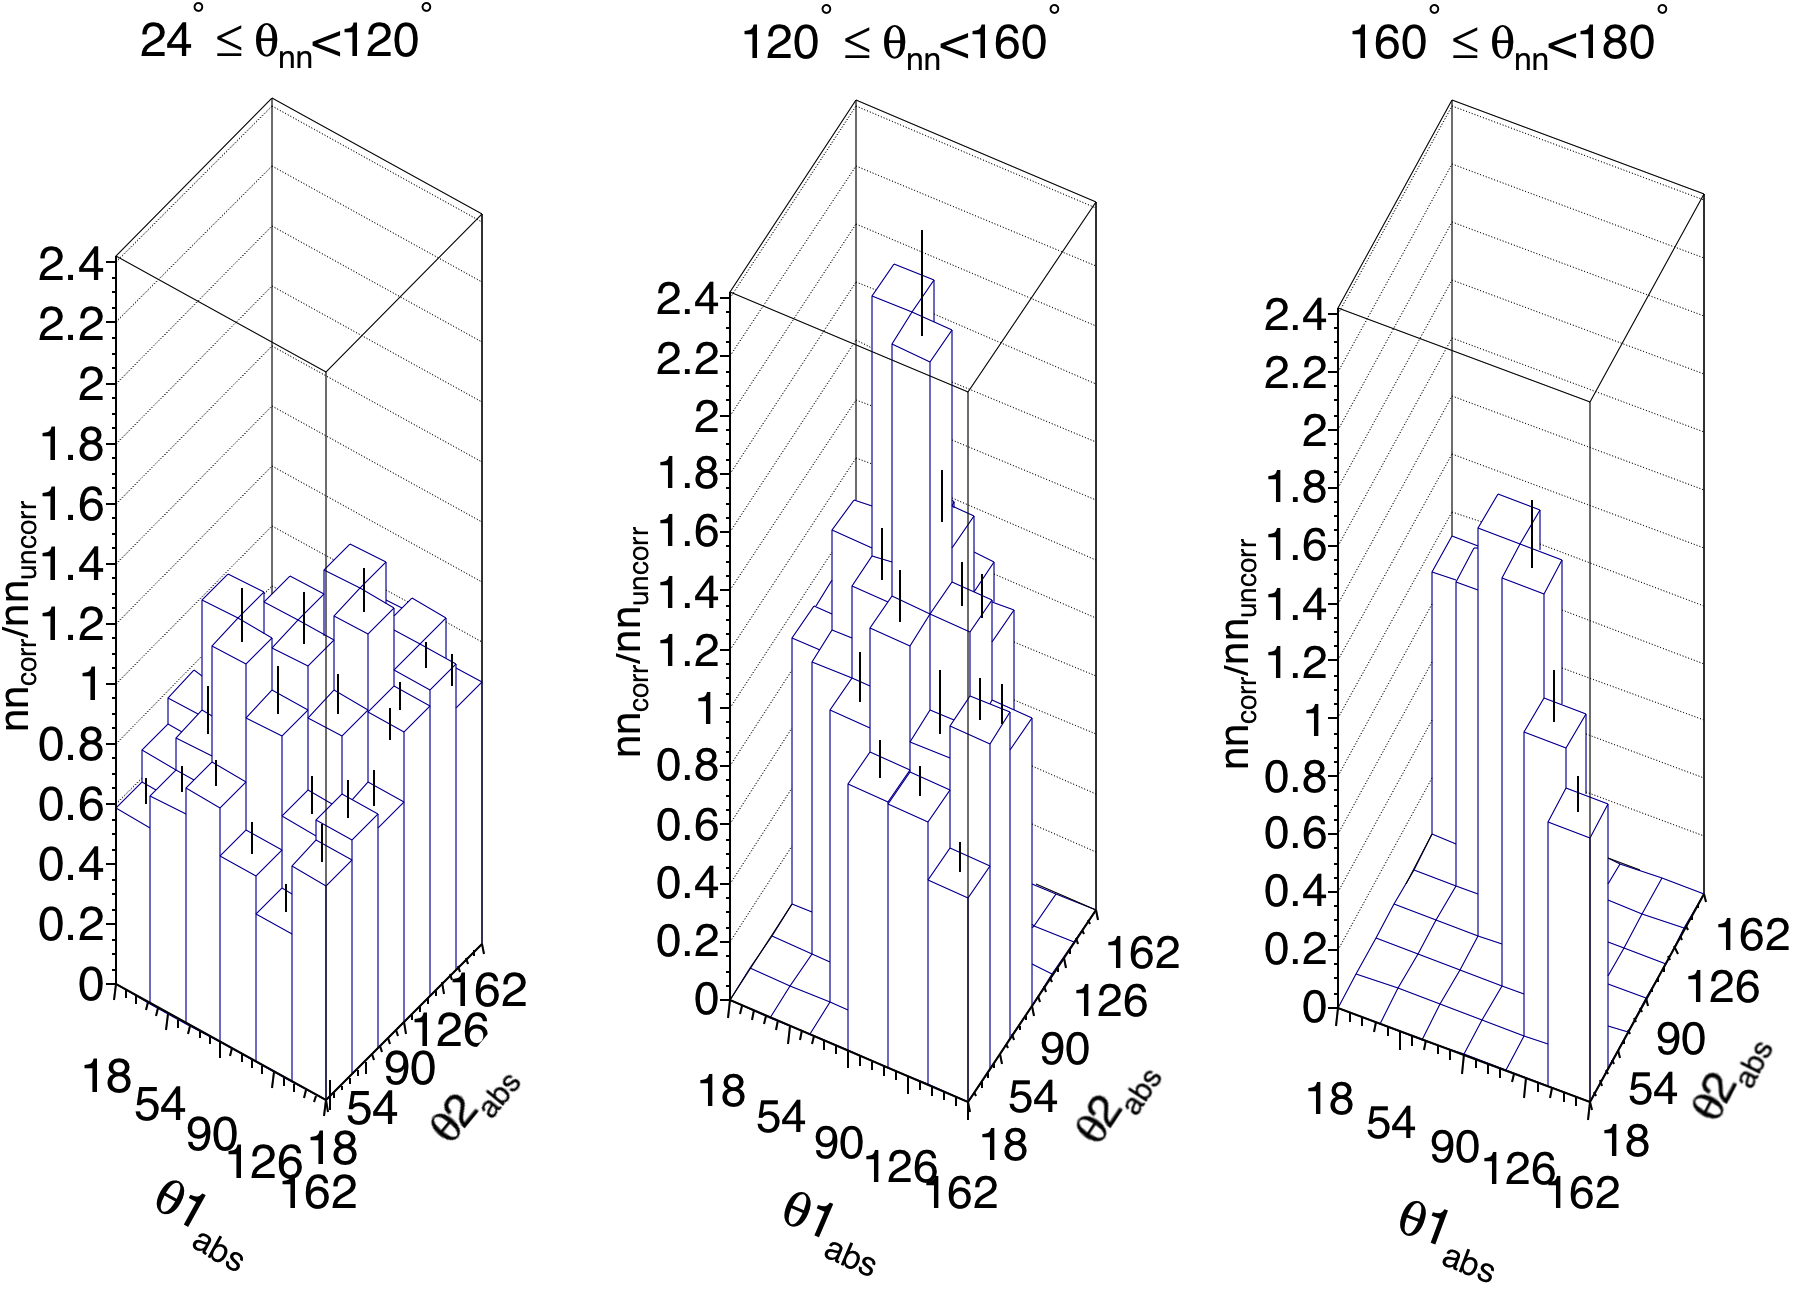
\includegraphics[width = 0.9\textwidth]{Content/Results/theta_abs_LEGO.png}
    \caption{Correlation is shown between the angles of each neutron with respect to the incident photon beam, denoted by $\theta 1_{abs}$ and $\theta 2_{abs}$.
    Empty bins exist because of incomplete $\theta_{abs}$ coverage.}
    \label{fig:theta_abs_LEGO}
\end{figure}
\begin{figure}
\centering
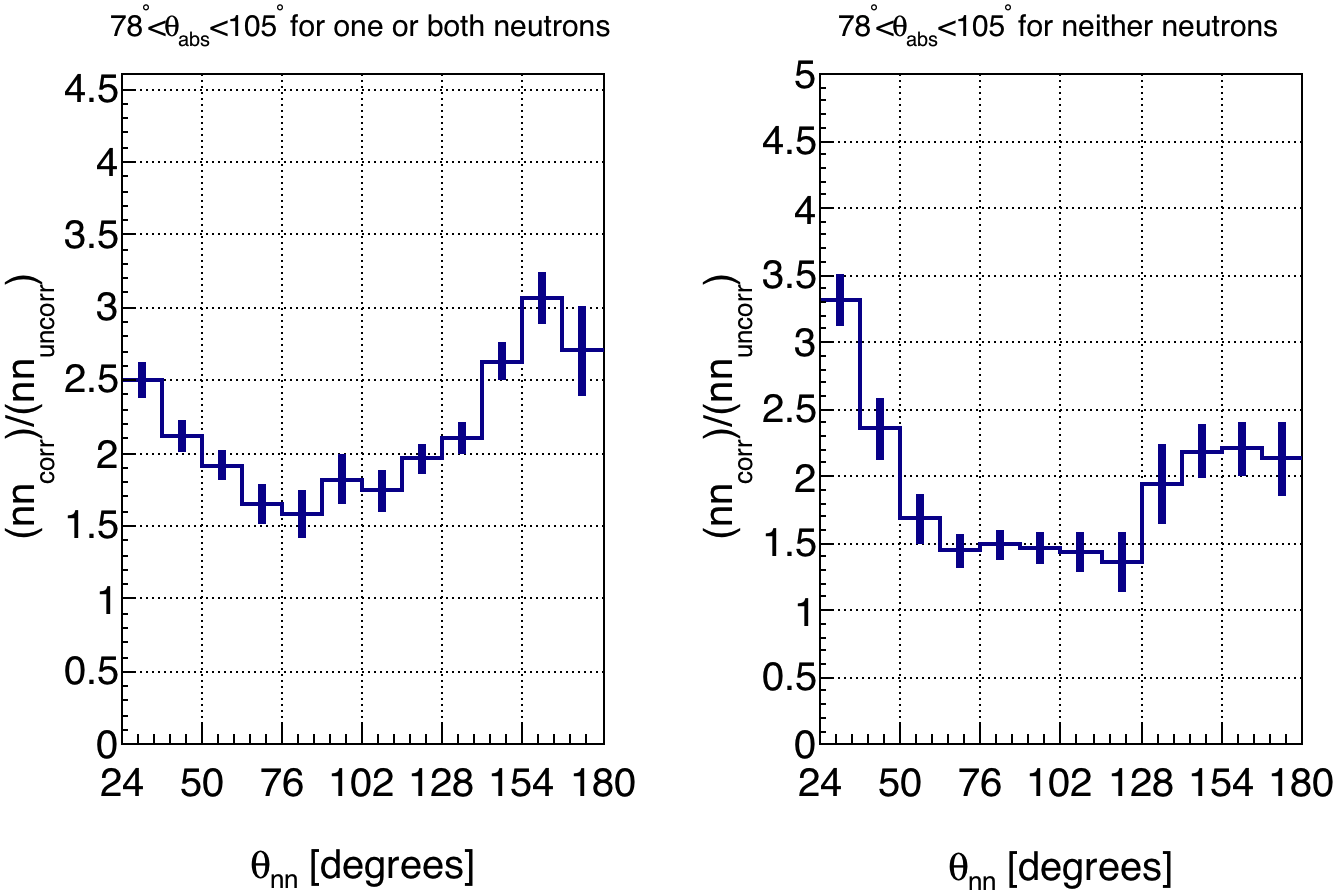
\includegraphics[width=0.9\textwidth]{Content/Results/theta_abs_two-neutron.png}
\caption{Requiring that at least one of the coincident neutrons be emitted nearly perpendicular to the photon beam (left) produces an opening angle distribution that is different from that produced when it is required that both neutrons are emitted nearly parallel to the photon beam (right).}
\label{fig:theta_abs_two_neutron}
\end{figure}
\FloatBarrier 

\section{Asymmetries in $\theta_{abs}$ of Neutron Singles}
Using data acquired during this study, it is possible to construct $\theta_{abs}$ distributions of neutron singles, where $\theta_{abs}$ is defined as the angle between a neutron's reconstructed direction of travel and the direction of the incident photon beam.
Because the experimental design was motivated by measurements of correlated neutron doubles and not neutron singles, the methods required to obtain a neutron singles measurement are far less robust than for neutron doubles.
Nonetheless, neutron singles measurements from the photo-disintegration of D$_{2}$O showed fair agreement with known values, so these results are not totally without merit.

The distributions were calculated by normalizing a yield of photo-neutrons to the yield of neutrons from SF of $^{252}$Cf, which have no preferred direction.
However, these two yields were measured under very different experimental conditions.
This is different from the case of n-n opening angle measurements, which uses the same set of neutron events to generate two yields--uncorrected yield and correlated yield.
Another difference for these measurements is that there is no uncorrelated yield to use to subtract undesirable signals from noise and photons.

 Due to differences in experimental conditions that existed during measurements of photo-neutrons and measurements of neutrons from the SF of $^{252}$Cf, there is a high potential for systematic errors.
The photo-neutron data must be corrected for detector dead-time, which, due to the presence of the photon beam, was about an order of magnitude higher for photo-neutron measurements than for $^{252}$Cf measurements.
Accidental coincidences caused by noise and photons was estimated from data taken with a non-neutron producing aluminum target, which had to also be corrected for dead-time, and, scaled to account for the fact that the aluminum and photo-neutron data sets have different gamma detection rates.
The result was then subtracted from the photo-neutron data.
Neutrons from the SF of $^{252}$Cf do not have the same energy distribution as photo-neutrons, which could lead to incorrect results.

Despite all this, the $\theta_{abs}$ distribution for D$_{2}$O agrees moderately well with the previously established distribution, but the same may not necessarily be true for $^{238}$U and $^{232}$Th, which have a signal-to-noise ratio that is about 7 and 100 times less than for D$_{2}$O, respectively.

\begin{figure}
    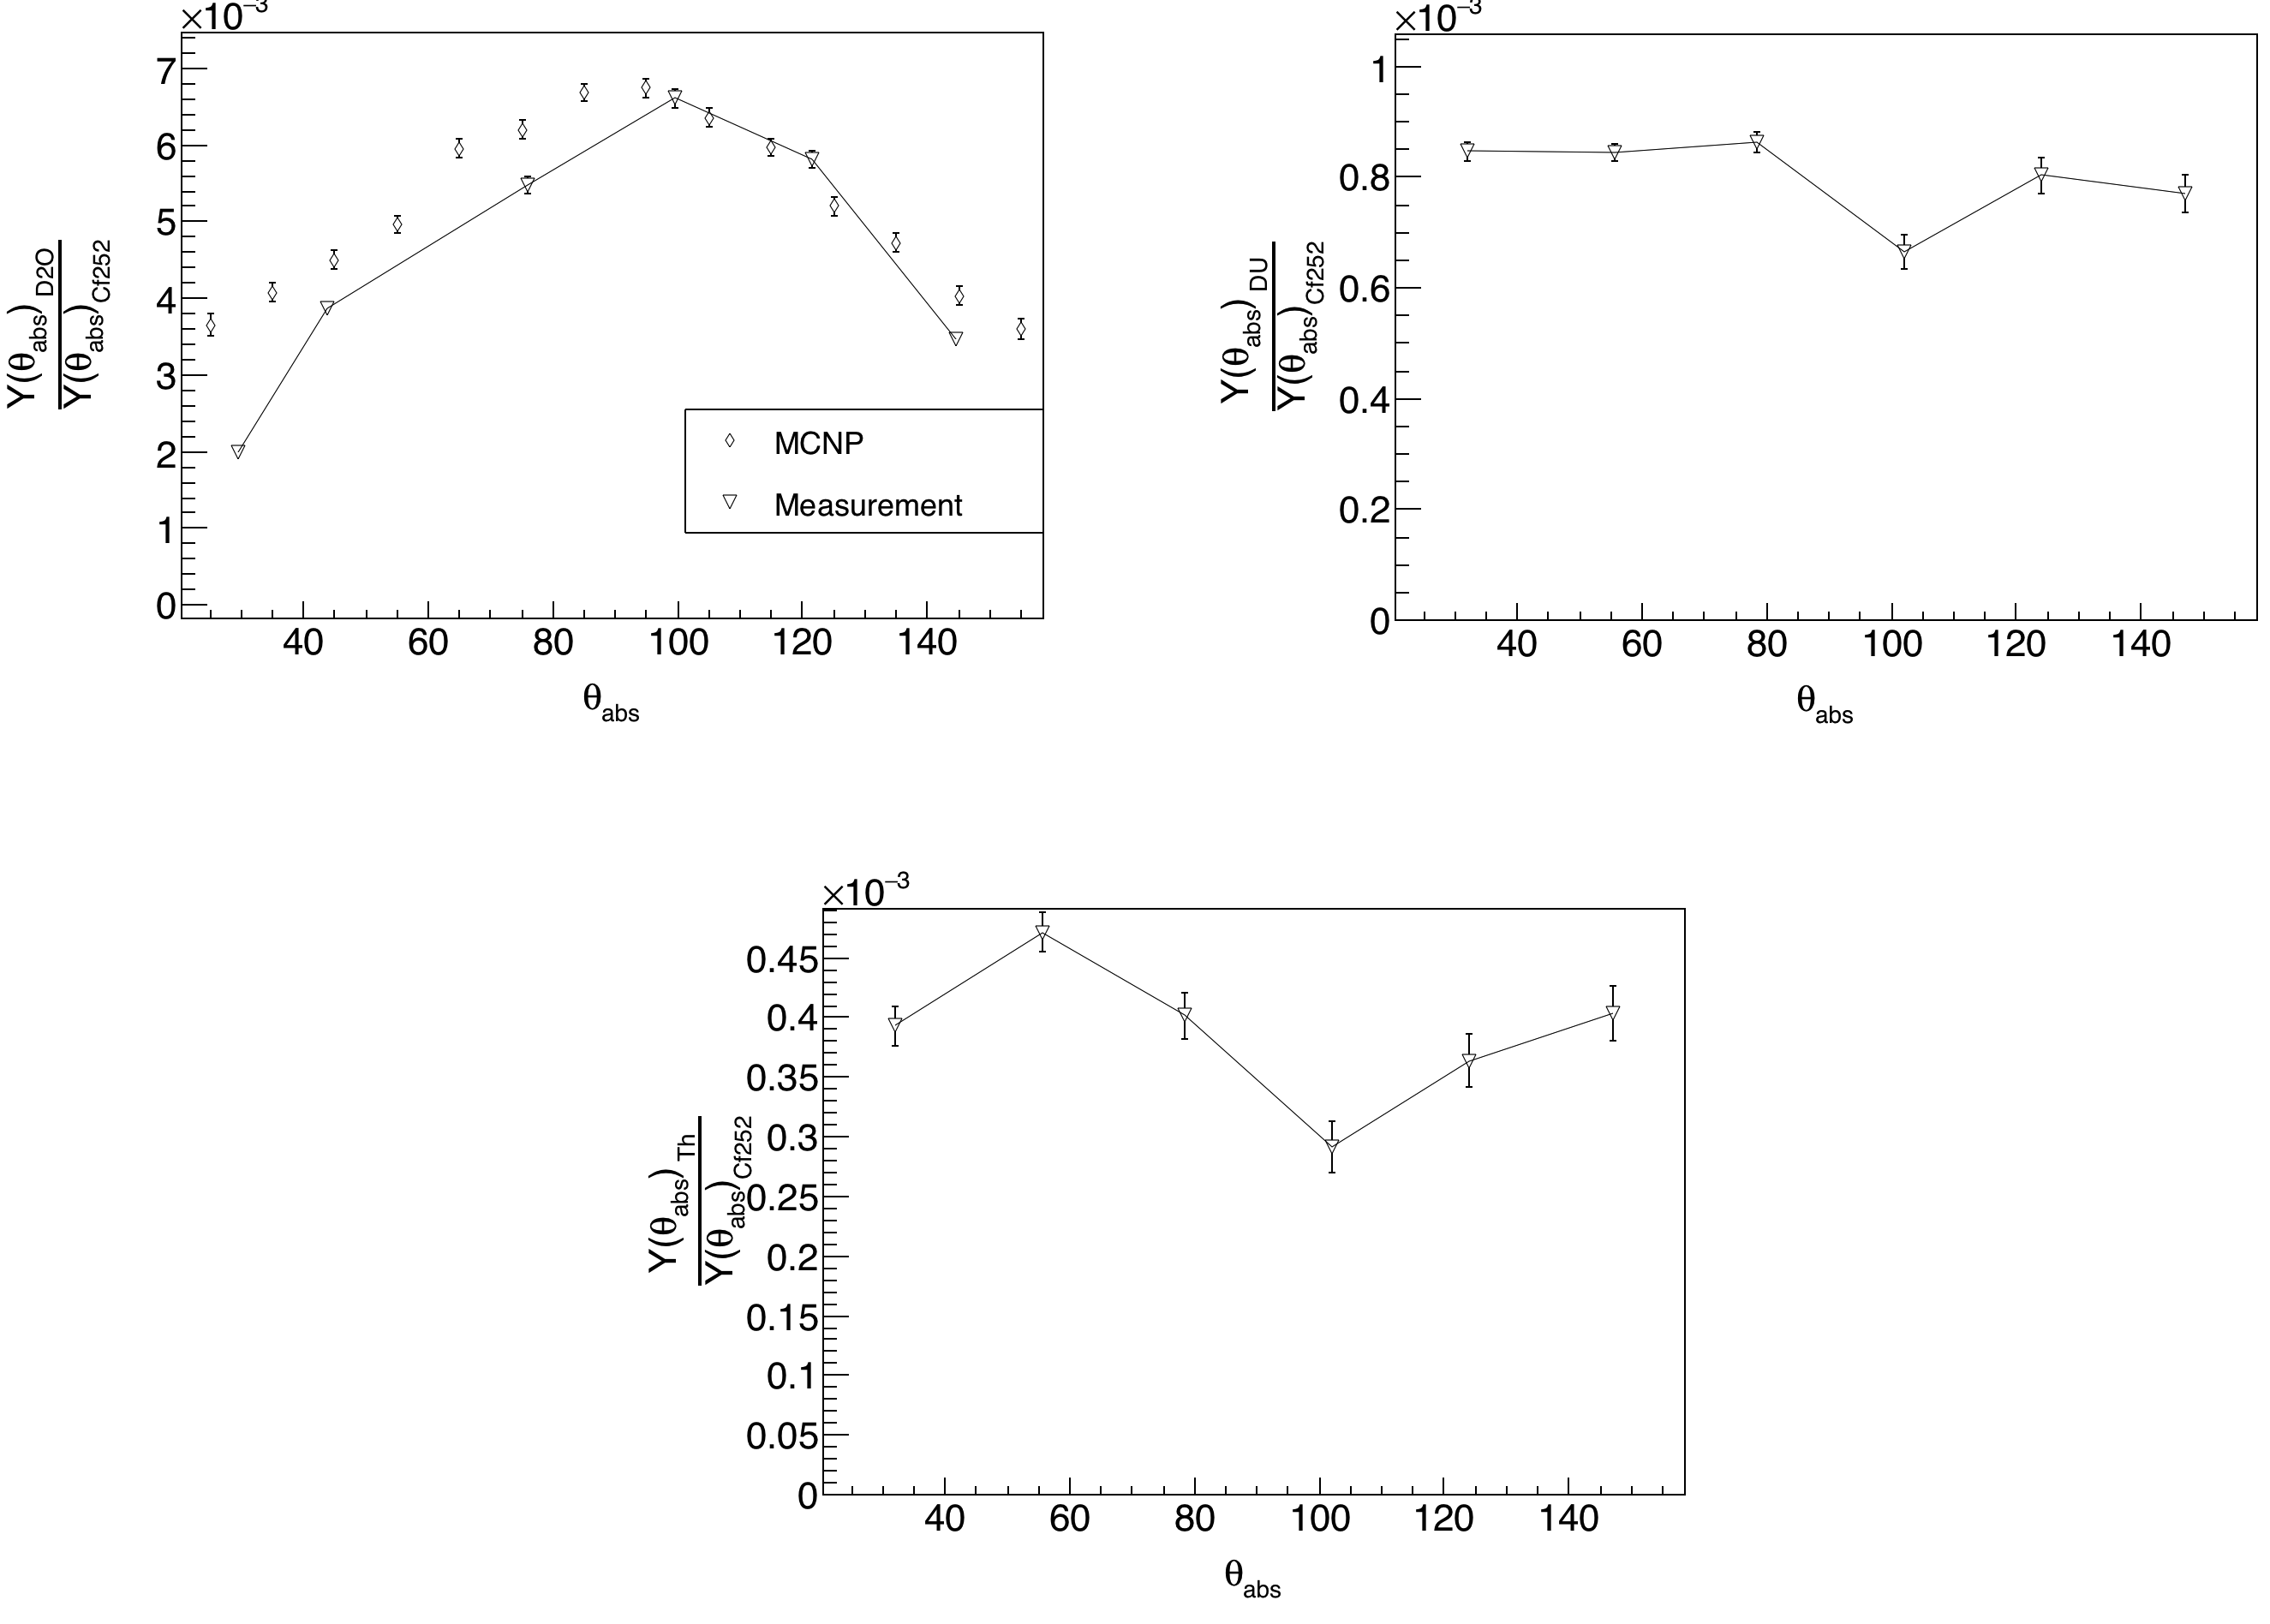
\includegraphics[width = 1\textwidth]{Content/Results/Singles.png}
    \caption{Accessory calculations were performed of the relative rates of neutrons singles as a function of $\theta_{abs}$. 
    Results are expressed as a ratio of the yield of photo-neutron singles from D$_{2}O$, $^{238}$U (DU), and $^{232}$Th, to the yield of neutron singles from the SF of $^{252}$Cf.
   The result for D$_{2}$O is in fair agreement with past measurements, however, these results have high potential for systematic errors due to the differences in experimental conditions under which the yields in the numerator and denominator (of the label for the y-axis) were measured.
       }
    \label{fig:Singles}
\end{figure}
\FloatBarrier